% !TeX TS-program = xelatex

\documentclass{resume}
\ResumeName{田润泽}

% 如果想插入照片,请使用以下两个库。
% \usepackage{graphicx}
% \usepackage{tikz}

\begin{document}

\ResumeContacts{
  (+86)186-2569-8616,%
  \ResumeUrl{mailto:trunzer@ruc.edu.cn}{trunzer@ruc.edu.cn},%
  \ResumeUrl{https://trunzer-world.cn}{trunzer-world.cn} \footnote{下划线内容包含超链接。},%
  \ResumeUrl{https://github.com/Welldefine}{github.com/Welldefine}%
}

% 如果想插入照片,请取消此代码的注释。
% 但是默认不推荐插入照片,因为这不是简历的重点。
% 如果默认的照片插入格式不能满足你的需求,你可以尝试调整照片的大小,或者使用其他的插入照片的方法。
% 不然,也可以先渲染 PDF 简历,然后用其他工具在 PDF 上叠加照片。
% \begin{tikzpicture}[remember picture, overlay]
%   \node [anchor=north east, inner sep=1cm]  at (current page.north east) 
%      {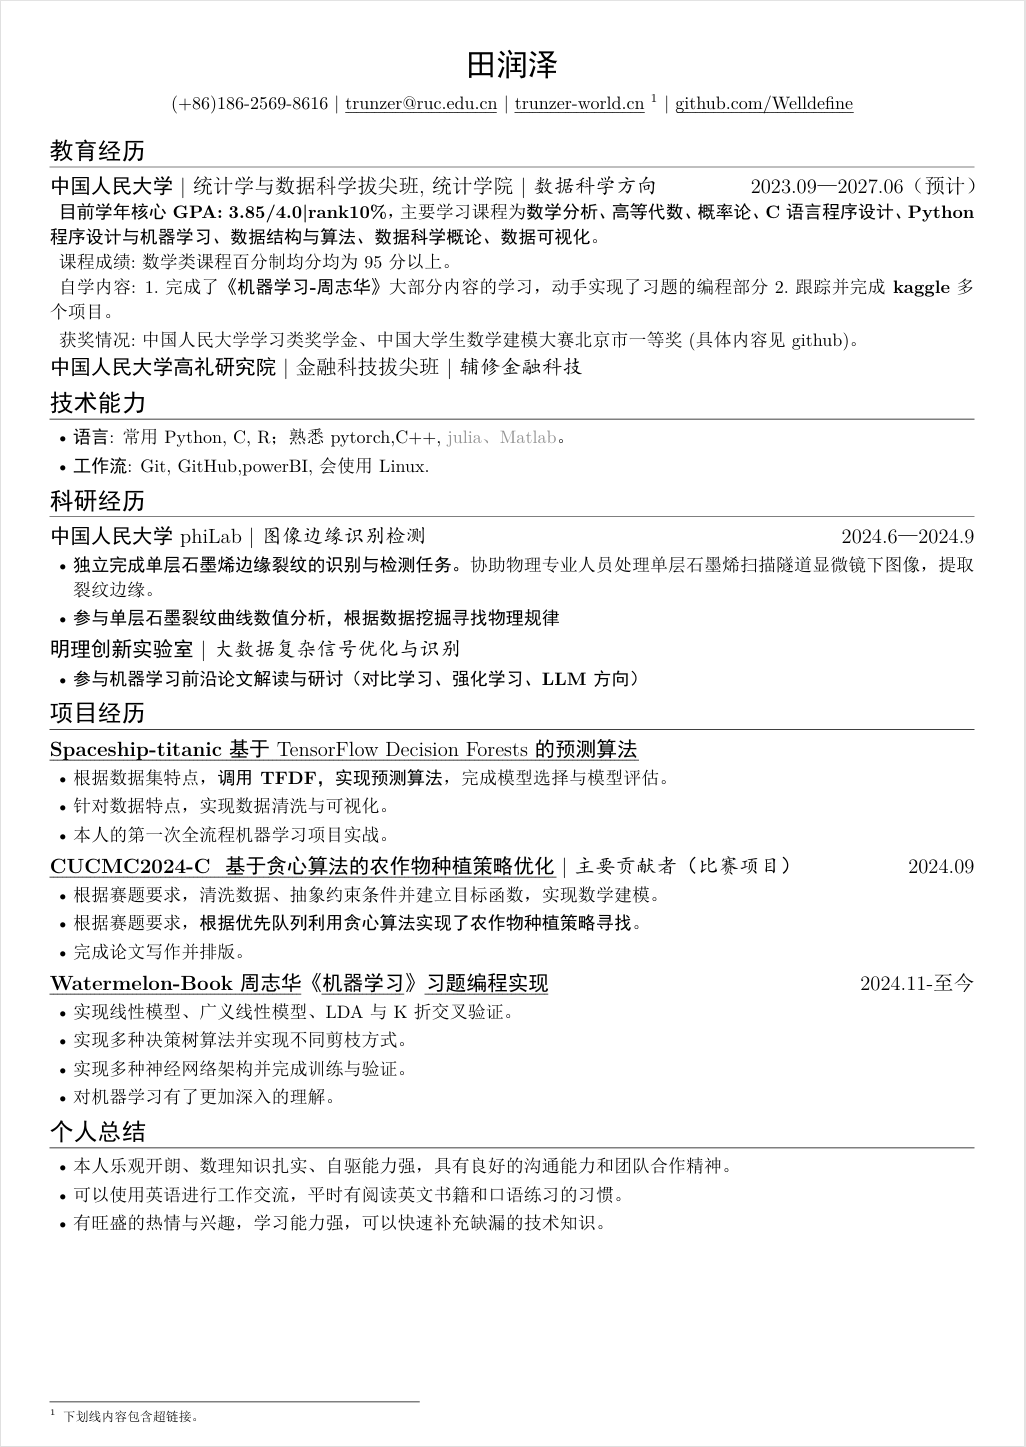
\includegraphics[width=2cm]{image.png}};
% \end{tikzpicture}

\ResumeTitle


\section{教育经历}
\ResumeItem
[中国人民大学|本科二年级在读]
{中国人民大学}
[\textnormal{统计学与数据科学拔尖班,统计学院|} 数据科学方向]
[2023.09—2027.06(预计)]

\textbf{目前学年核心GPA: 3.85/4.0|rank10\%},主要学习课程为\textbf{数学分析、高等代数、概率论、C语言程序设计、Python程序设计与机器学习、数据结构与算法、数据科学概论、数据可视化}。

课程成绩:数学类课程百分制均分均为95分以上。

自学内容: 1.完成了\textbf{《机器学习-周志华》}大部分内容的学习,动手实现了习题的编程部分
2.跟踪并完成\textbf{kaggle}多个项目。

获奖情况:中国人民大学学习类奖学金、中国大学生数学建模大赛北京市一等奖(具体内容见github)。
\ResumeItem
{中国人民大学高礼研究院}[\textnormal{金融科技拔尖班|} 辅修金融科技]


\section[技术能力]{技术能力\protect}
\begin{itemize}
  \item \textbf{语言}: 常用 Python, C, R; 熟悉 pytorch,C++, \GrayText{julia、Matlab}。
  \item \textbf{工作流}: Git, GitHub,powerBI,会使用Linux.
\end{itemize}

\section{科研经历}

\ResumeItem{中国人民大学phiLab}
[图像边缘识别检测]
[2024.6—2024.9] 

\begin{itemize}
  \item \textbf{独立完成单层石墨烯边缘裂纹的识别与检测任务。}协助物理专业人员处理单层石墨烯
  扫描隧道显微镜下图像,提取裂纹边缘。
  \item \textbf{参与单层石墨裂纹曲线数值分析,根据数据挖掘寻找物理规律}
\end{itemize}

\ResumeItem{明理创新实验室}
[大数据复杂信号优化与识别]
\begin{itemize}
  \item \textbf{参与机器学习前沿论文解读与研讨(对比学习、强化学习、LLM方向)}
\end{itemize}

\section{项目经历}

\ResumeItem[Spaceship-titanic 基于TensorFlow Decision Forests的预测算法]
{\ResumeUrl{https://www.kaggle.com/code/trunzer/spaceship-titanic-with-tfdf}{\textbf{Spaceship-titanic} 基于TensorFlow Decision Forests的预测算法}}

\begin{itemize}
  \item 根据 数据集特点,\textbf{调用TFDF,实现预测算法},完成模型选择与模型评估。
  \item 针对数据特点,实现数据清洗与可视化。
  \item 本人的第一次全流程机器学习项目实战。
\end{itemize}

\ResumeItem[CUCMC2024-C 基于贪心算法的农作物种植策略优化]
{\ResumeUrl{https://github.com/Welldefine/CUMCM2024-C}{\textbf{CUCMC2024-C } 基于贪心算法的农作物种植策略优化}}
[主要贡献者(比赛项目)]
[2024.09]

\begin{itemize}
  \item 根据赛题要求,清洗数据、抽象约束条件并建立目标函数,实现数学建模。
  \item 根据赛题要求,\textbf{根据优先队列利用 贪心算法 实现了农作物种植策略寻找}。
  \item 完成论文写作并排版。
\end{itemize}

\ResumeItem[Watermelon-Book 周志华《机器学习》习题编程实现]
{\ResumeUrl{https://github.com/Welldefine/Watermelon-Book}{\textbf{Watermelon-Book} 周志华《机器学习》习题编程实现}}
[]
[2024.11-至今]
\begin{itemize}
  \item 实现线性模型、广义线性模型、LDA与K折交叉验证。
  \item 实现多种决策树算法并实现不同剪枝方式。
  \item 实现多种神经网络架构并完成训练与验证。
  \item 对机器学习有了更加深入的理解。
\end{itemize}

\section{个人总结}

\begin{itemize}
  \item 本人乐观开朗、数理知识扎实、自驱能力强,具有良好的沟通能力和团队合作精神。
  \item 可以使用英语进行工作交流,平时有阅读英文书籍和口语练习的习惯。
  \item 有旺盛的热情与兴趣,学习能力强,可以快速补充缺漏的技术知识。
\end{itemize}


\end{document}
